% Standalone source of the figure fig:block of the coupling-integrals paper: the geometry of the coupling
% block, Eq. (eq:block).
% Build: pdflatex fig_block.tex; the paper includes the PDF. Grey scale only: line styles, not colour.
% (a) A source cell n and a field cell m in an oblique projection (receding axis to the upper right, as in
% fig_neighbours), offset o = (2, 0, 1) so that every quantity can be labelled; units of h, cube side 2.
% (b) A section through the centres of two cells in face contact, o = (1, 0, 0).
\documentclass[border=2pt]{standalone}
% Shared preamble of the standalone figures of the coupling-integrals paper.
\usepackage{amsmath,amssymb,bm}
\usepackage{tikz}
\usetikzlibrary{calc,arrows.meta}
\newcommand{\bR}{\mathbf{R}}
\newcommand{\bs}{\mathbf{s}}
\newcommand{\bu}{\mathbf{u}}
\newcommand{\bx}{\mathbf{x}}

\usetikzlibrary{decorations.pathmorphing,decorations.pathreplacing}
\newcommand{\bxi}{\bm{\xi}}
\newcommand{\bo}{\mathbf{o}}
\newcommand{\bP}{\mathbf{P}}
% projection of the point (x, y, z): x to the right, y receding to the upper right, z up
\newcommand{\pt}[3]{({(#1) + 0.45*(#2)}, {(#3) + 0.32*(#2)})}
% \cell{cx}{cy}{cz}{fill}: the cube of half-width 1 centred at (cx, cy, cz), see-through, with its hidden
% edges dotted
\newcommand{\cell}[4]{%
  \fill[#4, fill opacity=0.55]
    \pt{#1-1}{#2-1}{#3-1} -- \pt{#1+1}{#2-1}{#3-1} -- \pt{#1+1}{#2+1}{#3-1} -- \pt{#1+1}{#2+1}{#3+1}
    -- \pt{#1-1}{#2+1}{#3+1} -- \pt{#1-1}{#2-1}{#3+1} -- cycle;
  \draw[densely dotted, black!60]
    \pt{#1-1}{#2+1}{#3-1} -- \pt{#1+1}{#2+1}{#3-1}
    \pt{#1-1}{#2+1}{#3-1} -- \pt{#1-1}{#2-1}{#3-1}
    \pt{#1-1}{#2+1}{#3-1} -- \pt{#1-1}{#2+1}{#3+1};
  \draw[line join=round]
    \pt{#1-1}{#2-1}{#3-1} -- \pt{#1+1}{#2-1}{#3-1} -- \pt{#1+1}{#2-1}{#3+1} -- \pt{#1-1}{#2-1}{#3+1} -- cycle
    \pt{#1-1}{#2-1}{#3+1} -- \pt{#1-1}{#2+1}{#3+1} -- \pt{#1+1}{#2+1}{#3+1} -- \pt{#1+1}{#2-1}{#3+1}
    \pt{#1+1}{#2-1}{#3-1} -- \pt{#1+1}{#2+1}{#3-1} -- \pt{#1+1}{#2+1}{#3+1};
}
\begin{document}
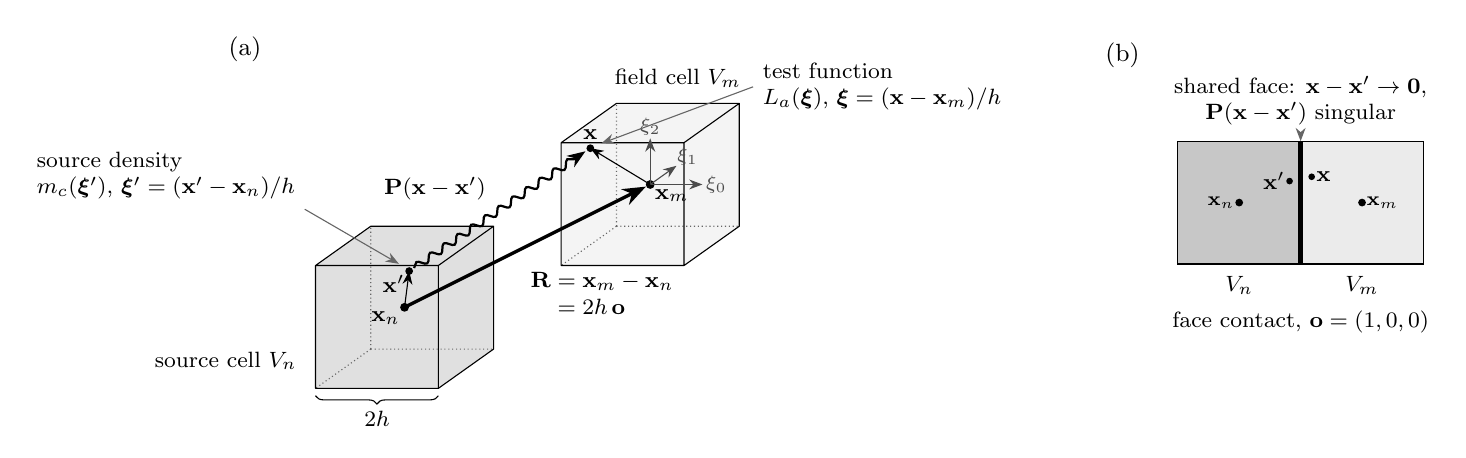
\begin{tikzpicture}[>=Stealth, x=0.78cm, y=0.78cm, font=\small]
  % ---------------------------------------------------------------- (a) the two cells and the integrand
  \begin{scope}
    \node at (-2.6,4.2) {(a)};
    \cell{0}{0}{0}{black!22}
    \cell{4}{0}{2}{black!8}
    \node[font=\footnotesize, anchor=east] at \pt{-1.15}{-1}{-0.55} {source cell $V_n$};
    \node[font=\footnotesize, anchor=south] at \pt{4}{1}{3.1} {field cell $V_m$};
    % side 2h, along the bottom front edge of the source cell
    \draw[decorate, decoration={brace, mirror, amplitude=3pt}] \pt{-1}{-1}{-1.12} -- \pt{1}{-1}{-1.12};
    \node[font=\footnotesize, anchor=north, inner sep=1pt] at \pt{0}{-1}{-1.32} {$2h$};
    % centres and their separation R = x_m - x_n = 2h o
    \fill \pt{0}{0}{0} circle (1.6pt);
    \node[font=\footnotesize, anchor=north east, inner sep=1.5pt] at \pt{0}{0}{0} {$\bx_n$};
    \fill \pt{4}{0}{2} circle (1.6pt);
    \node[font=\footnotesize, anchor=north west, inner sep=1.5pt] at \pt{4}{0}{2} {$\bx_m$};
    \draw[->, very thick] \pt{0}{0}{0} -- \pt{3.93}{0}{1.965};
    \node[font=\footnotesize, align=left, anchor=north west, fill=white, fill opacity=0.85, text opacity=1,
      inner sep=1pt] at \pt{2.0}{0}{0.62} {$\bR=\bx_m-\bx_n$\\ $\phantom{\bR}=2h\,\bo$};
    % local coordinates of the field cell: xi = (x - x_m)/h in [-1, 1]^3
    \draw[->, black!70] \pt{4}{0}{2} -- \pt{4.85}{0}{2} node[right, font=\scriptsize, inner sep=1pt] {$\xi_0$};
    \draw[->, black!70] \pt{4}{0}{2} -- \pt{4}{0.95}{2} node[above right, font=\scriptsize, inner sep=0pt] {$\xi_1$};
    \draw[->, black!70] \pt{4}{0}{2} -- \pt{4}{0}{2.75} node[above, font=\scriptsize, inner sep=1pt] {$\xi_2$};
    % a source point x' = x_n + h xi' and a field point x = x_m + h xi
    \draw[->, thin] \pt{0}{0}{0} -- \pt{0.3}{-0.5}{0.75};
    \fill \pt{0.3}{-0.5}{0.75} circle (1.4pt);
    \node[font=\footnotesize, anchor=north east, inner sep=1.5pt] at \pt{0.3}{-0.5}{0.75} {$\bx'$};
    \draw[->, thin] \pt{4}{0}{2} -- \pt{3.25}{-0.5}{2.75};
    \fill \pt{3.25}{-0.5}{2.75} circle (1.4pt);
    \node[font=\footnotesize, anchor=south, inner sep=2pt] at \pt{3.25}{-0.5}{2.8} {$\bx$};
    % the point propagator from the source point to the field point
    \draw[->, thick, decorate, decoration={snake, amplitude=1.3pt, segment length=6pt, post length=4pt}]
      \pt{0.38}{-0.5}{0.8} -- \pt{3.17}{-0.5}{2.7};
    \node[font=\footnotesize, anchor=south east, inner sep=1pt] at \pt{1.6}{-0.5}{1.85} {$\bP(\bx-\bx')$};
    % what each point carries
    \node[font=\footnotesize, align=left, anchor=east] (src) at \pt{-1.4}{-0.5}{2.3}
      {source density\\ $m_c(\bxi')$, $\bxi'=(\bx'-\bx_n)/h$};
    \draw[->, black!60, shorten >=3pt] (src.south east) -- \pt{0.25}{-0.5}{0.8};
    \node[font=\footnotesize, align=left, anchor=west] (fld) at \pt{5.9}{-0.5}{3.75}
      {test function\\ $L_a(\bxi)$, $\bxi=(\bx-\bx_m)/h$};
    \draw[->, black!60, shorten >=3pt] (fld.west) -- \pt{3.3}{-0.5}{2.78};
  \end{scope}
  % ---------------------------------------------------------------- (b) cells that touch: x - x' -> 0
  \begin{scope}[xshift=10.6cm, yshift=0.55cm]
    \node at (-1.9,3.4) {(b)};
    \fill[black!22] (-1,0) rectangle (1,2);
    \fill[black!8] (1,0) rectangle (3,2);
    \draw (-1,0) rectangle (1,2);
    \draw (1,0) rectangle (3,2);
    \draw[line width=1.6pt] (1,0) -- (1,2);
    \node[font=\footnotesize, anchor=north] at (0,-0.05) {$V_n$};
    \node[font=\footnotesize, anchor=north] at (2,-0.05) {$V_m$};
    \fill (0,1) circle (1.4pt) node[left, font=\scriptsize, inner sep=1.5pt] {$\bx_n$};
    \fill (2,1) circle (1.4pt) node[right, font=\scriptsize, inner sep=1.5pt] {$\bx_m$};
    % source and field points on either side of the shared face, nearly coincident
    \fill (0.82,1.35) circle (1.2pt) node[left, font=\footnotesize, inner sep=1.5pt] {$\bx'$};
    \fill (1.18,1.42) circle (1.2pt) node[right, font=\footnotesize, inner sep=1.5pt] {$\bx$};
    \node[font=\footnotesize, align=center, anchor=south] at (1,2.1)
      {shared face: $\bx-\bx'\to\mathbf0$,\\ $\bP(\bx-\bx')$ singular};
    \draw[->, black!60] (1,2.12) -- (1,2.0);
    \node[font=\footnotesize, align=center, anchor=north] at (1,-0.6)
      {face contact, $\bo=(1,0,0)$};
  \end{scope}
\end{tikzpicture}
\end{document}
